% \documentclass[compacto,10pt]{aleph-notas}
\documentclass[compacto,10pt,comentarios]{aleph-notas}

% -- Paquetes adicionales
\usepackage{enumitem}
\usepackage{aleph-comandos}
\usepackage{parskip}
\usepackage{graphicx}
\usepackage{xfrac}
\usepackage{tikz}
\usepackage{etoolbox}
% \AtBeginEnvironment{proof}{\color{white}}
\usepackage[framemethod=tikz]{mdframed}
\DeclareFontFamily{U}{skulls}{}
\DeclareFontShape{U}{skulls}{m}{n}{ <-> skull }{}
\newcommand{\skull}{\text{\usefont{U}{skulls}{m}{n}\symbol{'101}}}
\def \ds{\displaystyle}
\def \dfx{\dfrac{d}{dx}}
\DeclareMathOperator{\arccot}{arccot}
\DeclareMathOperator{\arcsec}{arcsec}
\DeclareMathOperator{\arccsc}{arccsc}

% -- Datos del libro
\institucion{Southwestern College}
\asignatura{MATH 251: Calculus II}
\tema{Arc Length}
\autor{Jesús Pérez Cuarenta}
% \fecha{Fall 2024}

%% --> Logos de las guias
\logouno[4.5cm]{../Images/swc_logo}
\definecolor{colordef}{cmyk}{0.81, 0.62, 0.00, 0.22}

\begin{document}

\encabezado

\section*{Arc Length}

Recall that the radian is a unit that is used to measure angles and one radian is the angle made at the center of a circle by an arc whose length is equal to the radius of the circle.

If we are not dealing with a circle, how can we find the length of a curve?

Suppose a curve is given by $y = f(x)$, where $f$ is a function with a continuous first derivative on the interval $[a,b]$.

\begin{figure}[h!]
\centering	
	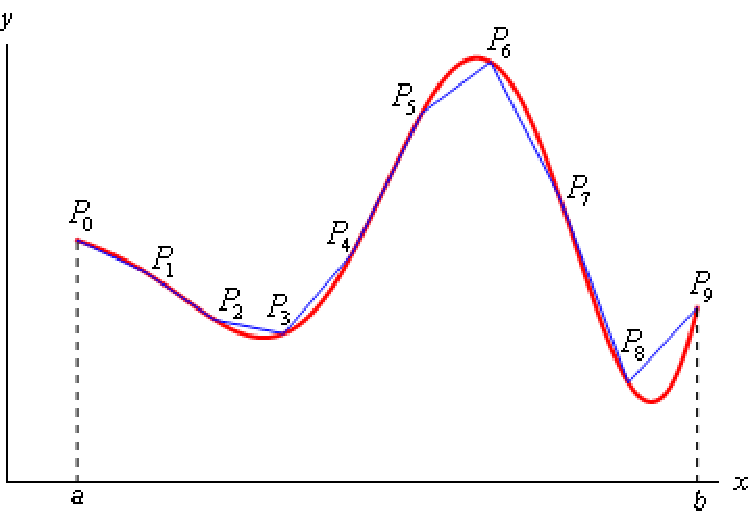
\includegraphics[width=0.7\linewidth]{../Images/6_5_arclength_01.pdf}
\end{figure}

The length $L$ of the curve will be 
$$
    L = \ds \lim_{n \to \infty}\sum_{i=1}^{n}|P_{i-1}P_i|
$$

We can use the distance formula find the length of the segments to get
$$
    \left| {{P_{i - 1}}\,\,{P_i}} \right| = \sqrt {{{\left( {{x_i} - {x_{i - 1}}} \right)}^2} + {{\left( {{y_i} - {y_{i - 1}}} \right)}^2}}  = \sqrt {\Delta {x^2} + \Delta y_i^2}
$$

By applying the Mean Value Theorem to $f$ on the interval $[x_{i-1}, x_i]$, we can see that there exists a number $x_i^* \in [x_{i - 1}, x_{i}]$ such that

$$
    f(x_i)-f(x_{i-1})= f'(x_i^*)(x_i-x_{i-1})
$$
i.e.,
$$
    \Delta y_i = f'(x_i^*) ~ \Delta x ~ .
$$

Thus, we have
\begin{align*}
	|P_{i-1}P_i|
    &= \sqrt{(\Delta x)^2+(\Delta y)^2} \\
    &=\sqrt{(\Delta x)^2+[f'(x_i^*)\Delta x]^2} \\
	&= \sqrt{1+[f'(x_i^*)]^2}\sqrt{(\Delta x)^2} \\
    &=  \sqrt{1+[f'(x_i^*)]^2} \Delta x .
\end{align*}
Therefore, 
$$
    L = \ds \lim_{n \to \infty} \sum_{i=1}^{n} |P_{i-1}P_i| = \lim_{n \to \infty} \sum_{i=1}^{n} \sqrt{1+[f'(x_i^*)]^2} \Delta x ~ .
$$


\begin{defi}[\textbf{Arc Length for $y = f(x)$}]
    Let $y = f(x)$ have a continuous first derivative on the interval $[a, b]$. The length of the curve from $\left(a, f(a)\right)$ to $\left(b, f(b)\right)$ is
    $$
        L = \int_{a}^{b} \sqrt{1 + \left( f'(x) \right) ^ {2}} dx.
    $$
\end{defi}

\begin{defi}[\textbf{Arc Length for $x = g(y)$}]
    Let $x = g(y)$ have a continuous first derivative on the interval $[c, d]$. The length of the curve from $\left(g(c), c\right)$ to $\left(g(d), d\right)$ is
    $$
        L = \int_{c}^{d} \sqrt{1 + \left( g'(y) \right) ^ {2}} dy.
    $$
\end{defi}

%%%%%%%%%%%%%%%%%%%%%%%%%%%%%%%%%%%%%%%%%%%%%%%%%%%%
%% Examples
%%%%%%%%%%%%%%%%%%%%%%%%%%%%%%%%%%%%%%%%%%%%%%%%%%%%
% \color{white}
\begin{ejer}
    Find the length of the curve 
    $$
        f(x) = x^{\sfrac{3}{2}}
    $$
    between $x=0$ and $x=4$.
\end{ejer}

\begin{proof}[Solution]
    We have
    \begin{align*}
        f'(x) = \frac{d}{dx} \left( x^{\sfrac{3}{2}} \right) = \frac{3}{2} x ^ {\sfrac{1}{2}}
    \end{align*}
    Using the definition of arc length we get 
    \begin{align*}
        L & = \int_{a}^{b} \sqrt{1 + \left( f'(x) \right) ^ {2}} ~ dx \\
        & = \int_{0}^{4} \sqrt{1 + \left( \frac{3}{2} x ^ {\sfrac{1}{2}} \right)^{2} } ~ dx \\
        & = \int_{0}^{4} \sqrt{1 + \frac{9}{4}x} ~ dx.
    \end{align*}
    Let $u = 1 + \frac{9}{4}x$, it  follows that
    $$
        \frac{du}{dx} = \frac{9}{4} \implies du = \frac{9}{4} ~ dx \iff \frac{4}{9} ~ du = dx.
    $$
    Hence,
    \begin{align*}
        \int_{0}^{4} \sqrt{1 + \frac{9}{4}x} ~ dx  & = \frac{4}{9} \int_{1}^{10} \sqrt{u} ~ du \\
        & = \left. \frac{4}{9} \cdot \frac{2}{3} u^{\sfrac{3}{2}} \right\rvert_{1}^{10} \\ 
        & = \frac{8}{27} \left( 10 ^ {\sfrac{3}{2}} - 1 ^ {\sfrac{3}{2} }\right) \\
        & = \frac{8}{27} \left( 10 \sqrt{10}  - 1 \right) .
    \end{align*}
\end{proof}

\begin{ejer}
    Find the length of the curve
    $$
        f(x) = 2e^{x} + \frac{1}{8}e^{-x}
    $$
    on the interval $[0, \ln{2}]$.
\end{ejer}
\begin{proof}[Solution]
    We have
    \begin{align*}
        f'(x) = \frac{d}{dx} \left(2e^{x} + \frac{1}{8}e^{-x} \right) = 2e^{x} - \frac{1}{8}e^{-x}
    \end{align*}
    Using the definition of arc length we get 
    \begin{align*}
        L & = \int_{a}^{b} \sqrt{1 + \left( f'(x) \right) ^ {2}} ~ dx \\
        & = \int_{0}^{\ln{2}} \sqrt{1 + \left( 2e^{x} - \frac{1}{8}e^{-x} \right)^{2} } ~ dx \\
        & = \int_{0}^{\ln{2}} \sqrt{1 + \left( 4e^{2x} - \frac{1}{2} + \frac{1}{64}e^{-2x} \right)} ~ dx \\
        & = \int_{0}^{\ln{2}} \sqrt{4e^{2x} + \frac{1}{2} + \frac{1}{64}e^{-2x}} ~ dx \\
        & = \int_{0}^{\ln{2}} \sqrt{\left(2e^{x} + \frac{1}{8} e^{-x}\right)^{2}} ~ dx \\
        & = \int_{0}^{\ln{2}} 2e^{x} + \frac{1}{8} e^{-x} ~ dx \\
        & = \left. \left( 2e^{x} - \frac{1}{8} e^{-x} \right) \right\rvert_{0}^{\ln{2}} \\
        & = \left( 2e^{\ln{2}} - \frac{1}{8} e^{-\ln{2}} \right) - \left( 2e^{0} - \frac{1}{8} e^{-0} \right) \\
        & = \frac{33}{16} ~ .
    \end{align*}
\end{proof}

\begin{ejer}
    Find the length of the curve
    $$
        x(y) = \dfrac{y^3}{6}+\dfrac{1}{2y}
    $$
    from $y = 1$ to $y = 2$. 
\end{ejer}
\begin{proof}[Solution]
    We have
    \begin{align*}
        x'(y) = \frac{d}{dy} \left( \dfrac{y^3}{6}+\dfrac{1}{2y} \right) = \frac{1}{2}y^{2} - \frac{1}{2y^{2}}
    \end{align*}
    Using the definition of arc length we get
    \begin{align*}
        L & = \int_{c}^{d} \sqrt{1 + \left( h'(x) \right) ^ {2}} ~ dy \\
        & = \int_{1}^{2} \sqrt{1 + \left(\frac{1}{2}y^{2} - \frac{1}{2y^{2}} \right)^{2}} ~ dy \\
        & = \int_{1}^{2} \sqrt{\frac{(y^{4} + 1)^{2}}{4y^{4}}} ~ dy \\
        & = \int_{1}^{2} \frac{y^{4} + 1}{2y^{2}} ~ dy \\
        & = \frac{1}{2} \int_{1}^{2} y^{2} + y^{-2} ~ dy \\
        & = \frac{1}{2} \left. \left( \frac{1}{3} y^{3} - y^{-1} \right) \right\rvert_{1}^{2} \\
        & = \frac{17}{12}.
    \end{align*}
\end{proof}

\begin{ejer}
    Given the following integral
    $$
        I = \int_{a}^{b} \sqrt{1 + 16x^{4}} ~ dx,
    $$
    provide examples of functions such that the arc length on the interval $[a, b]$ is determined by $I$.
\end{ejer}
\begin{proof}[Solution]
    Note that
    \begin{align*}
        I & = \int_{a}^{b} \sqrt{1 + 16x^{4}} ~ dx \\
        & = \int_{a}^{b} \sqrt{1 + (4x^{2})^{2}} ~ dx \\
        & = \int_{a}^{b} \sqrt{1 + (f'(x))^{2}} ~ dx .
    \end{align*}
    It is sufficient to produce $f(x)$ such that $f'(x) = 4x^{2}$. Namely,
    $$
        f(x) = \frac{4}{3} x ^{3} + C
    $$
    where $C \in \mathbb{R}$. Since $f(x)$ is a polynomial and polynomials are infinitely many times differentiable we are done. 
\end{proof}

\end{document}